\documentclass[12pt,letterpaper]{report}
\usepackage[utf8]{inputenc}
\usepackage[spanish]{babel}
\usepackage{amsmath}
\usepackage{amsfonts}
\usepackage{amssymb}
\usepackage{graphicx}
\usepackage[left=2cm,right=2cm,top=2cm,bottom=2cm]{geometry}
\author{Jose Antonio Olvera Gonzalez }
\title{Segundo Avance }
\begin{document}
\begin{center}
\textbf{Segundo Avance}
\begin{flushleft}
Descripcion del proyecto 
\begin{flushleft}
Este proyecto consiste en la realizacion de un robit esferico, los robots esféricos son capaces de desplazarse según diferentes trayectorias, pero suelen adolecer, en muchas ocasiones, de determinados inconvenientes, tales como que su movimiento no es continuo sino oscilatorio, complejo funcionamiento y control o necesidad de una precisión de fabricación del interior de la esfera que encarecerían su fabricación. Así, la presente invención se refiere a un robot esférico, en el que los medios de accionamiento son de constitución y funcionamiento sencillos, con un número reducido de componentes y que además permiten un desplazamiento tanto rectilíneo como curvilíneo, es decir, es capaz de desplazarse en diferentes sentidos y según trayectorias distintas, estando constituido por una carcasa esférica en la que se alojan medios de accionamiento que actúan sobre la superficie interna de dicha carcasa para provocar su desplazamiento. Además, este robot esférico asegura una actuación correcta de los medios de accionamiento, aunque la superficie interna de la carcasa esférica presente irregularidades.
\begin{flushleft}
Todas las articulaciones son de tipo rotacional. Se le denomina antropomórfico debido a las similitudes entre su estructura y el brazo humano. Estos robots tienen un gran espacio de trabajo y son muy populares, pero su control es mucho más complejo que el robot cartesiano, debido a su análisis dinámico. Se emplean en operaciones de ensamblaje, vaciado de metales, frezado, soldadura a gas, soldadura al arco, y pintura con spray.\\
\begin{center}
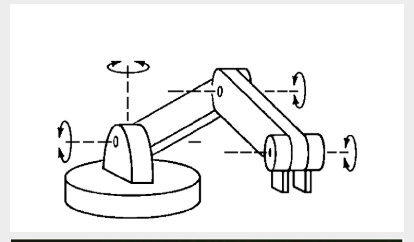
\includegraphics[scale=1]{1.PNG} 
\begin{flushleft}
Las primeras dos articulaciones son de tipo rotacional, en tanto que la tercera es de tipo prismática. El término de configuración esférica se debe al hecho de que son justamente las coordenadas esféricas, o polares, las que mejor definen la posición del efector terminal de este tipo de robots, con respecto a un sistema de referencia. Se usan en el manejo de máquinas-herramientas, soldaduras por puntos, vaciado de metales, frezado, soldadura a gas, y soldadura al arco.\\
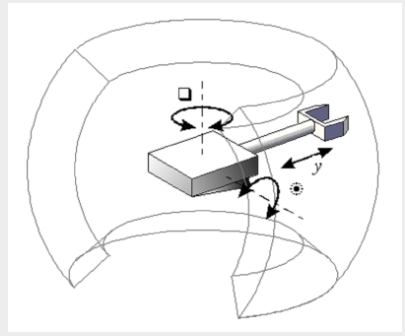
\includegraphics[scale=1]{2.PNG} 
\begin{flushleft}
Basandose en los ejemplos anteriores se prosedio al diceño en inventor para tener una mejor vision sobre el proyecto, ver dimenciones medidas angulos etc.\\
\begin{center}
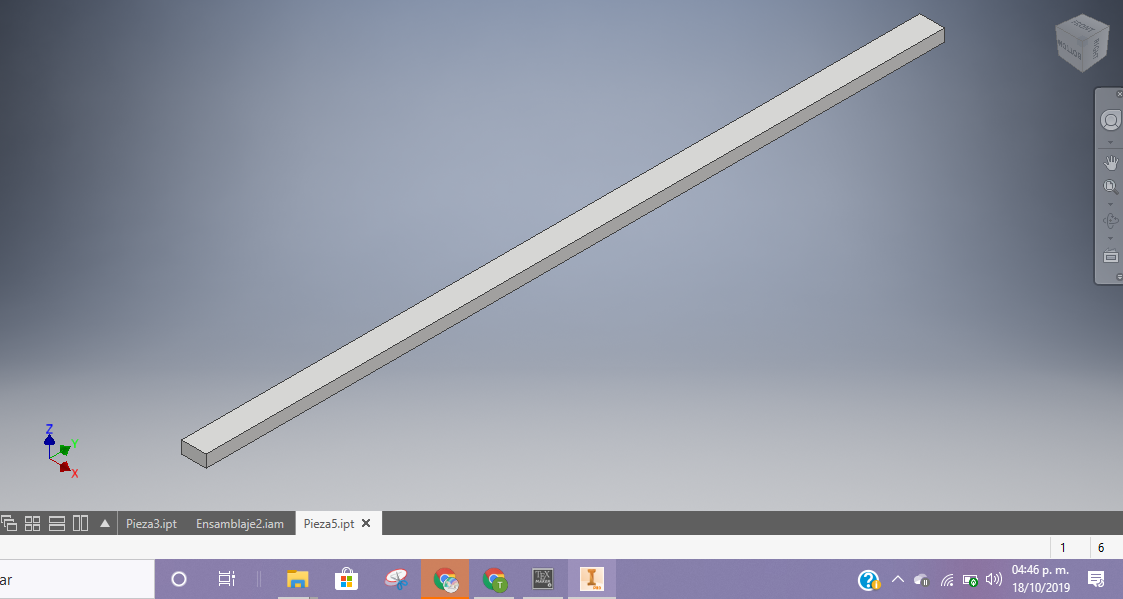
\includegraphics[scale=1]{3.PNG} \\
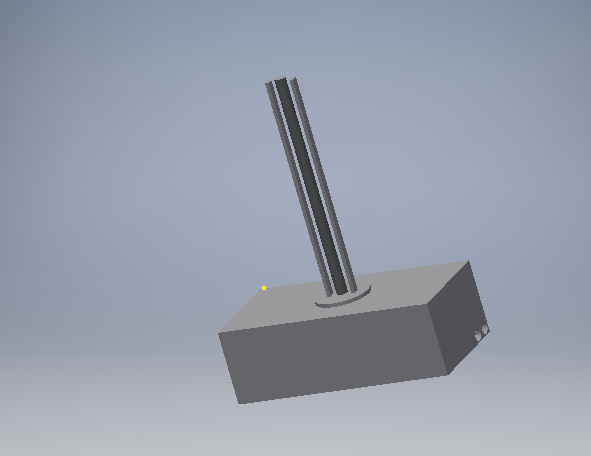
\includegraphics[scale=1]{4.PNG} 
\begin{flushleft}
Autodesk Inventor es el programa para diseño mecánico avanzado en 3D, con modelado paramétrico, directo y libre, tiene una capacidad base para realizar diseño de piezas, sus dibujos y ensambles de partes. En una versión profesional, Inventor ofrece simulación por elementos finitos, sistemas de movimientos, chapa metálica, ruteo de cables, plástico, moldes y administración de datos.
\begin{flushleft}
Ventajas de proyecto
\begin{flushleft}
-Tamaño pequeño frente a otros robots del mercado, lo que hace que pueda introducirse en sitios de dimensiones reducidas.\\
-Su movimiento se produce en cualquier dirección del plano y su movimiento es uniforme y controlado, pudiendo realizar giros sin problemas.\\
-El control del movimiento del robot se lleva a cabo de una manera muy sencilla, siendo fácil su implantación.

\end{flushleft}
\end{flushleft}
\end{flushleft}
\end{center}
\end{flushleft}
\end{flushleft}
\end{center}
\end{flushleft}
\end{flushleft}
\end{flushleft}
\end{center}
\end{document}